% Copyright 2024- Jay Jay Billings. Some rights reserved.
\documentclass{article}
\usepackage{graphicx} % Required for inserting images
\usepackage{hyperref}
\usepackage{tabularx}

\title{Learning to weld}
\author{Jay Jay Billings, Ph.D.}
\date{\today}

\begin{document}

\maketitle

I recently joined \href{https://makersmiths.org/}{Makersmiths}, a community forge and makerspace. I heard about Makersmiths in passing before moving to northern Virginia, and I was as happy as a school kid when I found that the Purcellville shop was close to my house after we moved. My wife and I put it on our list to join, and recently, she urged me to sign up when I started talking about building a bridge to cross our creek. I'll cover the bridge in a later blog, but I need to construct a bridge big enough to support my tractor across a 17-32ft span, depending on where I build the bridge. This will require some hefty steel, fin plates, huge bolts, and a lot of welding.

I won't cover Makersmiths in detail here, mainly because it is thoroughly discussed on our excellent website and \href{https://makersmiths.org/Blog}{blog}. But I really want to share what I learned in an excellent three-hour welding class on metal-inert gas welding that I finished last week! 

My first experience with welding was using a ``stick'' welder in my Dad's junkyard as a kid. We rarely used a welder because we were mostly cutting things to length for the smelter. Cutting was straightforward - and really fun! - using a reciprocating saw, a chop saw, or an oxyacetylene torch. Dad was masterful with the torch and was allegedly a superb welder, according to everyone in the yard. One fine day, he proved it and then gave us boys a quick lesson. Fast forward... a rather long time... and all I've done with welding since is simulate melt pools for work (arguably quite cool). I have soldered quite a bit, but any similarity between the physics of those two processes is outweighed by the difference in scale, in my opinion. So, when the metal inert gas welding course came up so soon after we joined, it looked like an excellent opportunity to get a jump start on building the skills I'll need to make the bridge.

\section*{Metal Inert Gas Welding}

You're probably familiar with stick welding, formally known as shielded metal arc welding, which uses a special metal electrode (or stick) coated (shielded) with a flux and an electrical arc to melt the pieces being welded. The metal electrode causes a short circuit between the metal and electrical ground of the welder, and the flux protects the welding melt pool/puddle from contamination or oxidation due to contact with air. The metal electrode melts and fills the gap between the pieces, welding them into a single piece.

Metal Inert Gas (MIG) welding is another type of electrical arc welding. Instead of using a stick for the electrode, it uses a wire, and instead of using a flux, it uses an inert gas. As long as a small trigger is pressed, the welder continuously feeds the wire and the inert gas through the gun and onto the surface of the material. MIG welding feels a lot more like using the world's most dangerous caulk or glue gun because of how it ejects material directly from the end of the gun, versus stick welding, which has the stick pointing in a different direction than the positive electrode that the welder is holding.

\subsection*{The Equipment}

I worked with three main types of equipment in my welding adventure: the plasma cutter, the MIG welder, and my new welding clothes. (We will get to why the clothing is just as important as the rest in due time.) Makersmith's has a nice welding shop that was partially stocked by a generous donation from Lincoln Electric that included welders, clothing and helmets, a plasma cutter, and fume extractors. General welding tools such as pliers, clamps, brushes, wire, etc. are all provided in the welding shop too.

\subsubsection*{Plasma Cutter}

We made coupons from 10-gauge steel strips using Makersmith's Lincoln Electric Tomahawk 375 Air Plasma Cutter. Plasma cutters are just about the neatest cutters on the planet and more or less live up to that old ``hot knife through butter'' adage. I cut six coupons from two fifteen-inch strips.

\subsubsection*{MIG Welder}

I decided to lump the metal welding table, fire bricks, and crow's feet (for making electrical connections between the table and things on the bricks) into the welder section because they wouldn't be there if not for the welder. The table is metal to act as a conductive path between the part and the ground of the welder, which is connected to the table if the part is too small. The part is placed on a fire brick to prevent it from welding to the table and thick wire crows feet bridge the table and part across the brick.

The welder I used was the Lincoln Electric 210mp MIG welder that comes with a fully interactive display. The on-board computer will calculate the necessary wire feed rate and voltage based on your material and wire thickness. The user can manually override these settings with a dial to preferred or better settings based on the weld. I used 0.030'' wire with C25 (75\% argon, 25\% carbon dioxide) gas.

It isn't exactly germane, but I found the ``Ready. Set. Weld.'' slogan displayed when the welder is booting is quite comical and a nice touch. The other nice touch about this welder is that the parameter chart is posted inside the wire chamber for easy access.

\subsubsection*{Clothes}

While there are lots of ads and videos on the internet showing people wearing, shall we say, \textit{less} clothing while welding, that's not how it works. Clothing is extremely important when welding to protect the welder from harm, which can include multiple types of burning, electrocution, abrasion, laceration, and blunt force trauma. UV skin burns, molten metal burns, and electrocution are high on the list. 

I was clad head to toe in my red wing steel-toed boots, Dickie's coveralls, a welding shirt, leather gloves, a welding helmet, and a pirate dew rag (to protect my bald head with a little walk-the-plank pizzaz). I went so heavy on the clothes after watching a \href{https://www.youtube.com/watch?v=2hAJJky4KAQ}{``Top 5 ways to die from welding'' video by ``Auto Expert John Cadogan'' on YouTube}. I was most surprised by the risk of skin burns from UV because I did not know that a significant amount of UV radiation was produced in the electrical arc during welding. The ``metal flash burn,'' as it is sometimes called, causes burns worse than a typical sunburn in only a few minutes of exposure. Luckily, I learned this a few days before the course, so I had time to order a few extra things from Amazon.

\section*{Welds}

\href{https://docs.google.com/document/d/1sYnxE0w3G5uM2nR5jFW012oVzhfzPJhmpwZoW4EnWKo/edit#heading=h.kmv1drr7rapm}{The Makersmiths MIG Welding Basics course} is three hours and starts with a presentation on welding, basic safety, the equipment, and the work ahead. After that, students learn to use the plasma cutter to create the coupons. In my course, we did both test cuts and welds before working with the actual material. Once the coupons are cut, students perform three welds: a butt joint, a corner joint, and a T-joint.

When I was welding, I wanted to focus on control over full coverage. I also stopped a lot to evaluate what I was doing and whether it seemed to work. This helped me learn how to see the weld path next to the bright melt pool, which I found initially challenging. I have a lot of learning left to do, but I'm happy with what I brought home.

\subsection*{Butt Weld}

The first ``real'' weld I attempted was a simple butt weld of two coupons, shown in figures \ref{butt1} and \ref{butt2}. I performed this weld at the default feed rate of 280 in/min and voltage of 19V. Welding from left to right, my first weld was too fast to fully penetrate the coupons. The second, third, and fourth attempts penetrated the material, but the third and fourth bits deposited significant material on the back side of the plate (shown in figure \ref{butt2}).

\begin{figure}[h]
\caption{Front side of my butt weld. The weld path goes from left to right.}
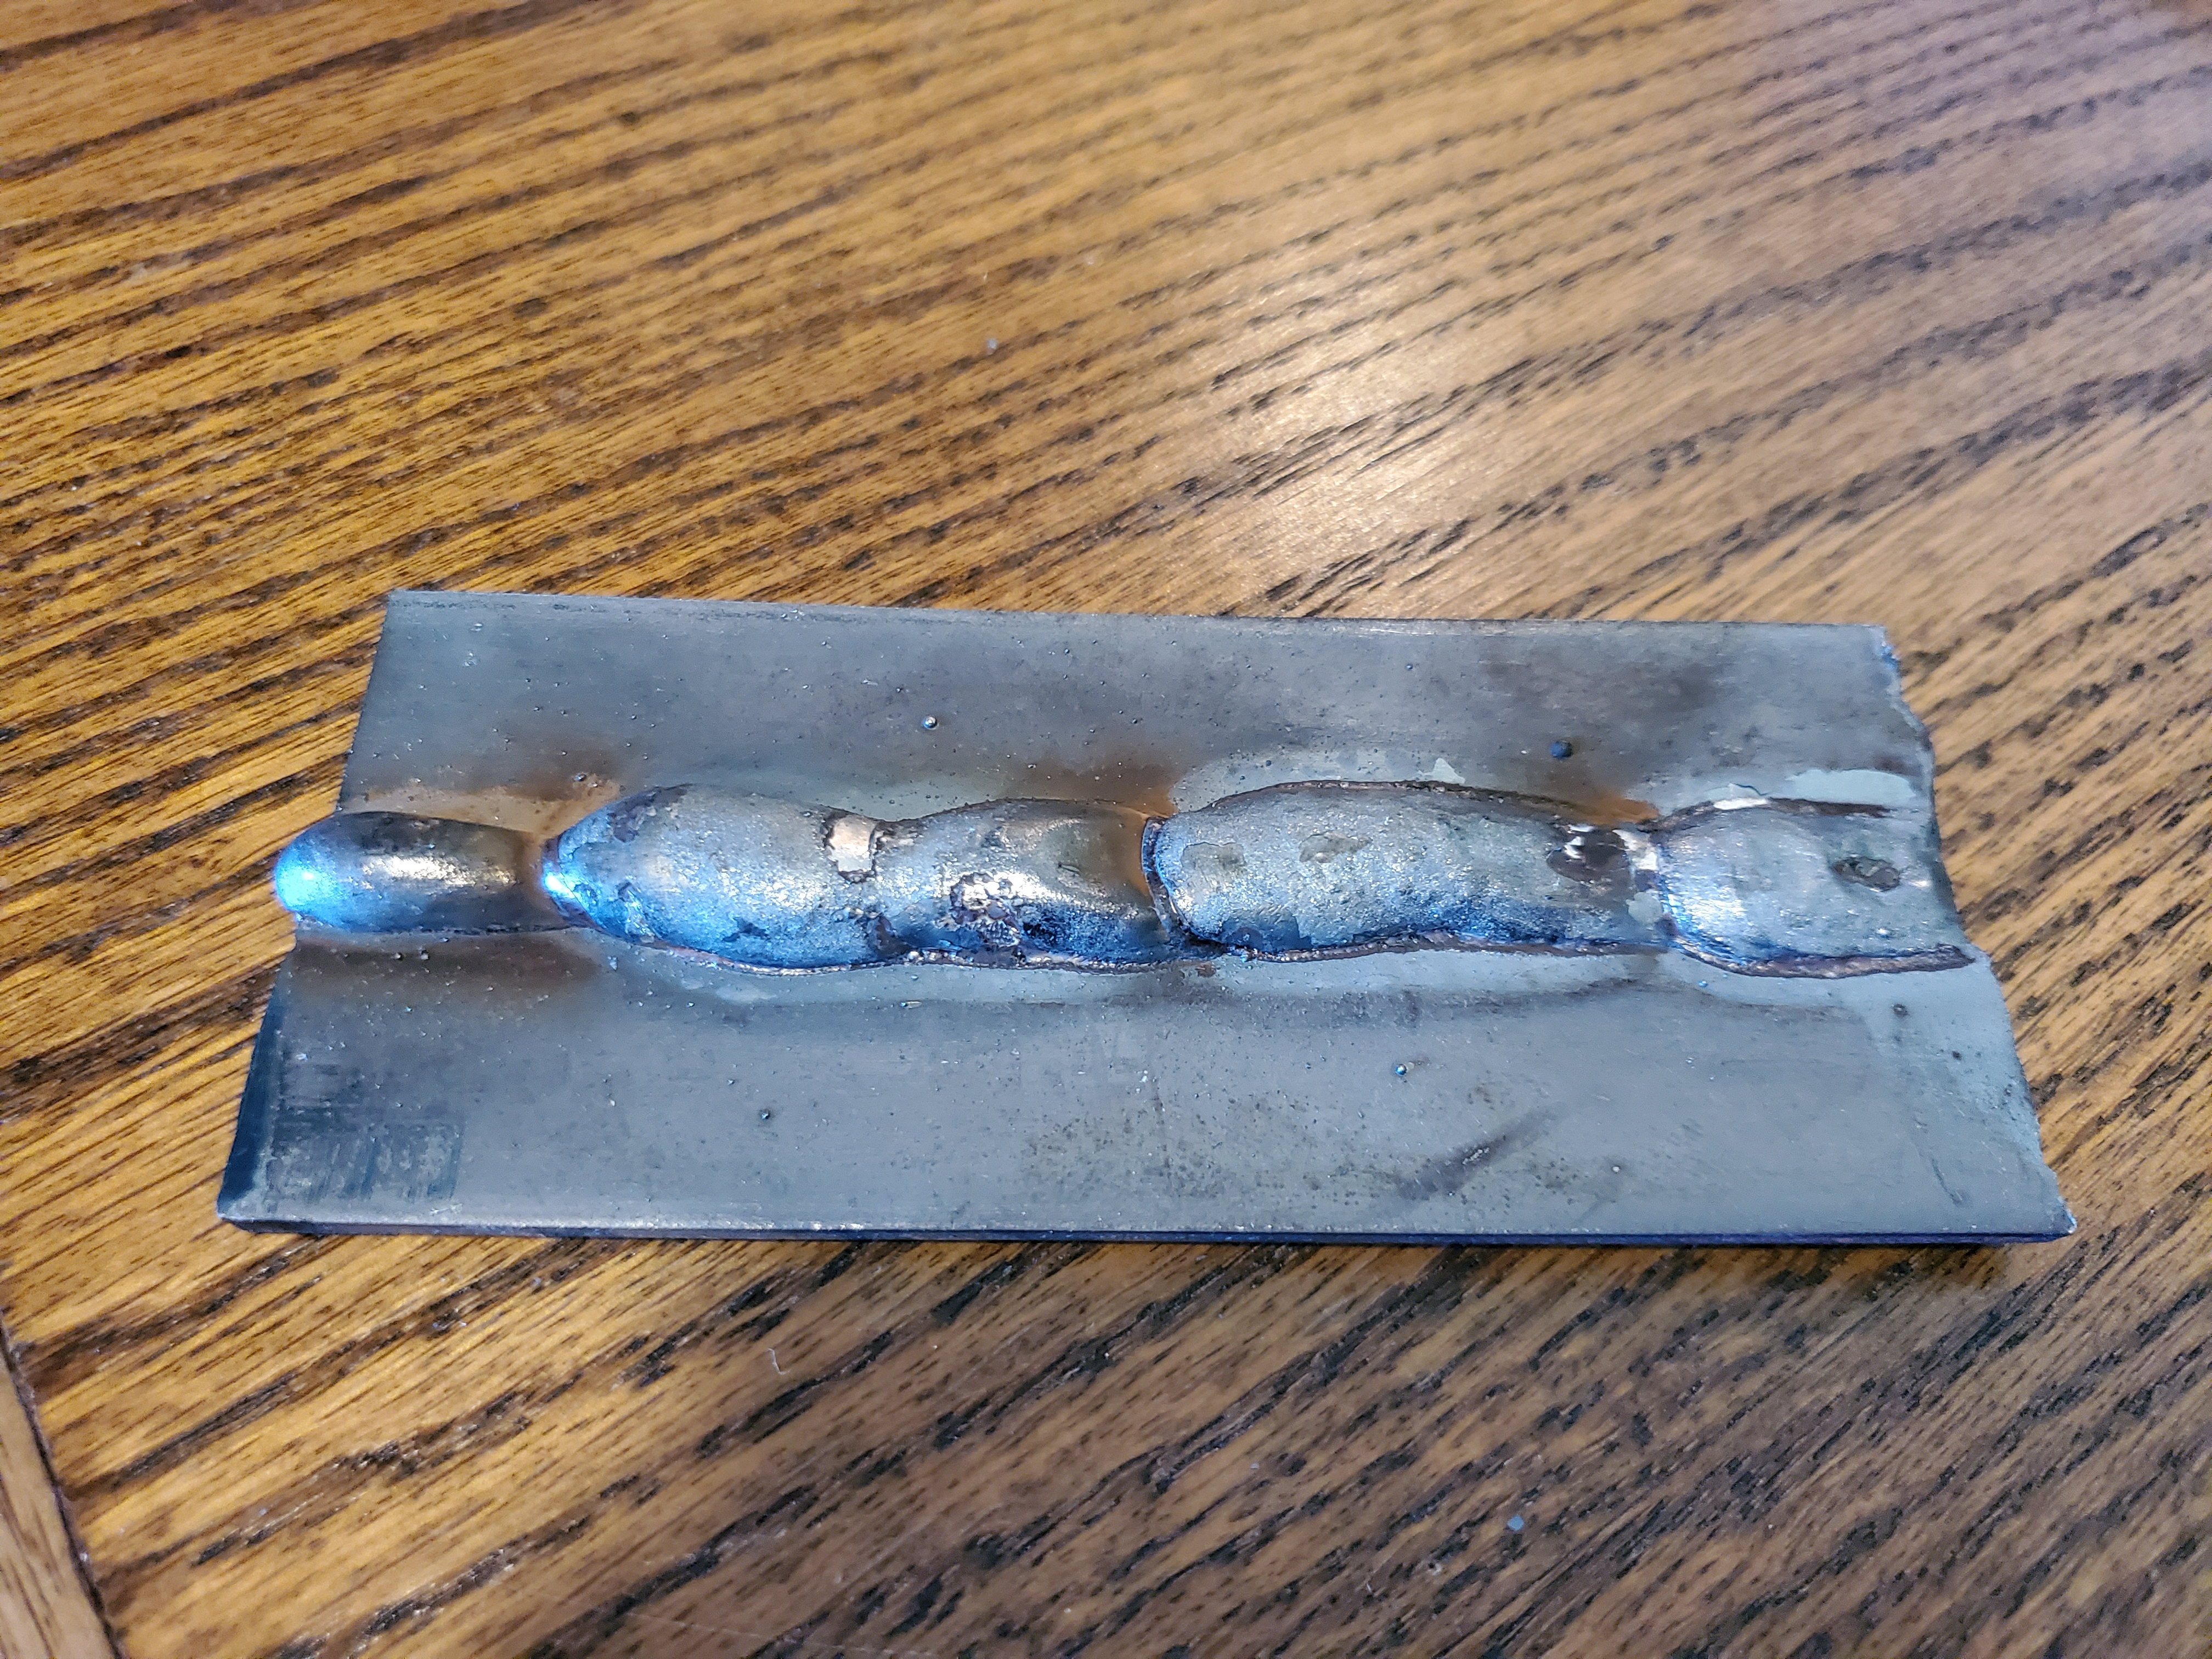
\includegraphics[width=\textwidth]{assets/buttWeldFront_20240229.jpg}
\label{butt1}
\end{figure}

\begin{figure}[h]
\caption{Back side of my butt weld with the weld path going from left to right.}
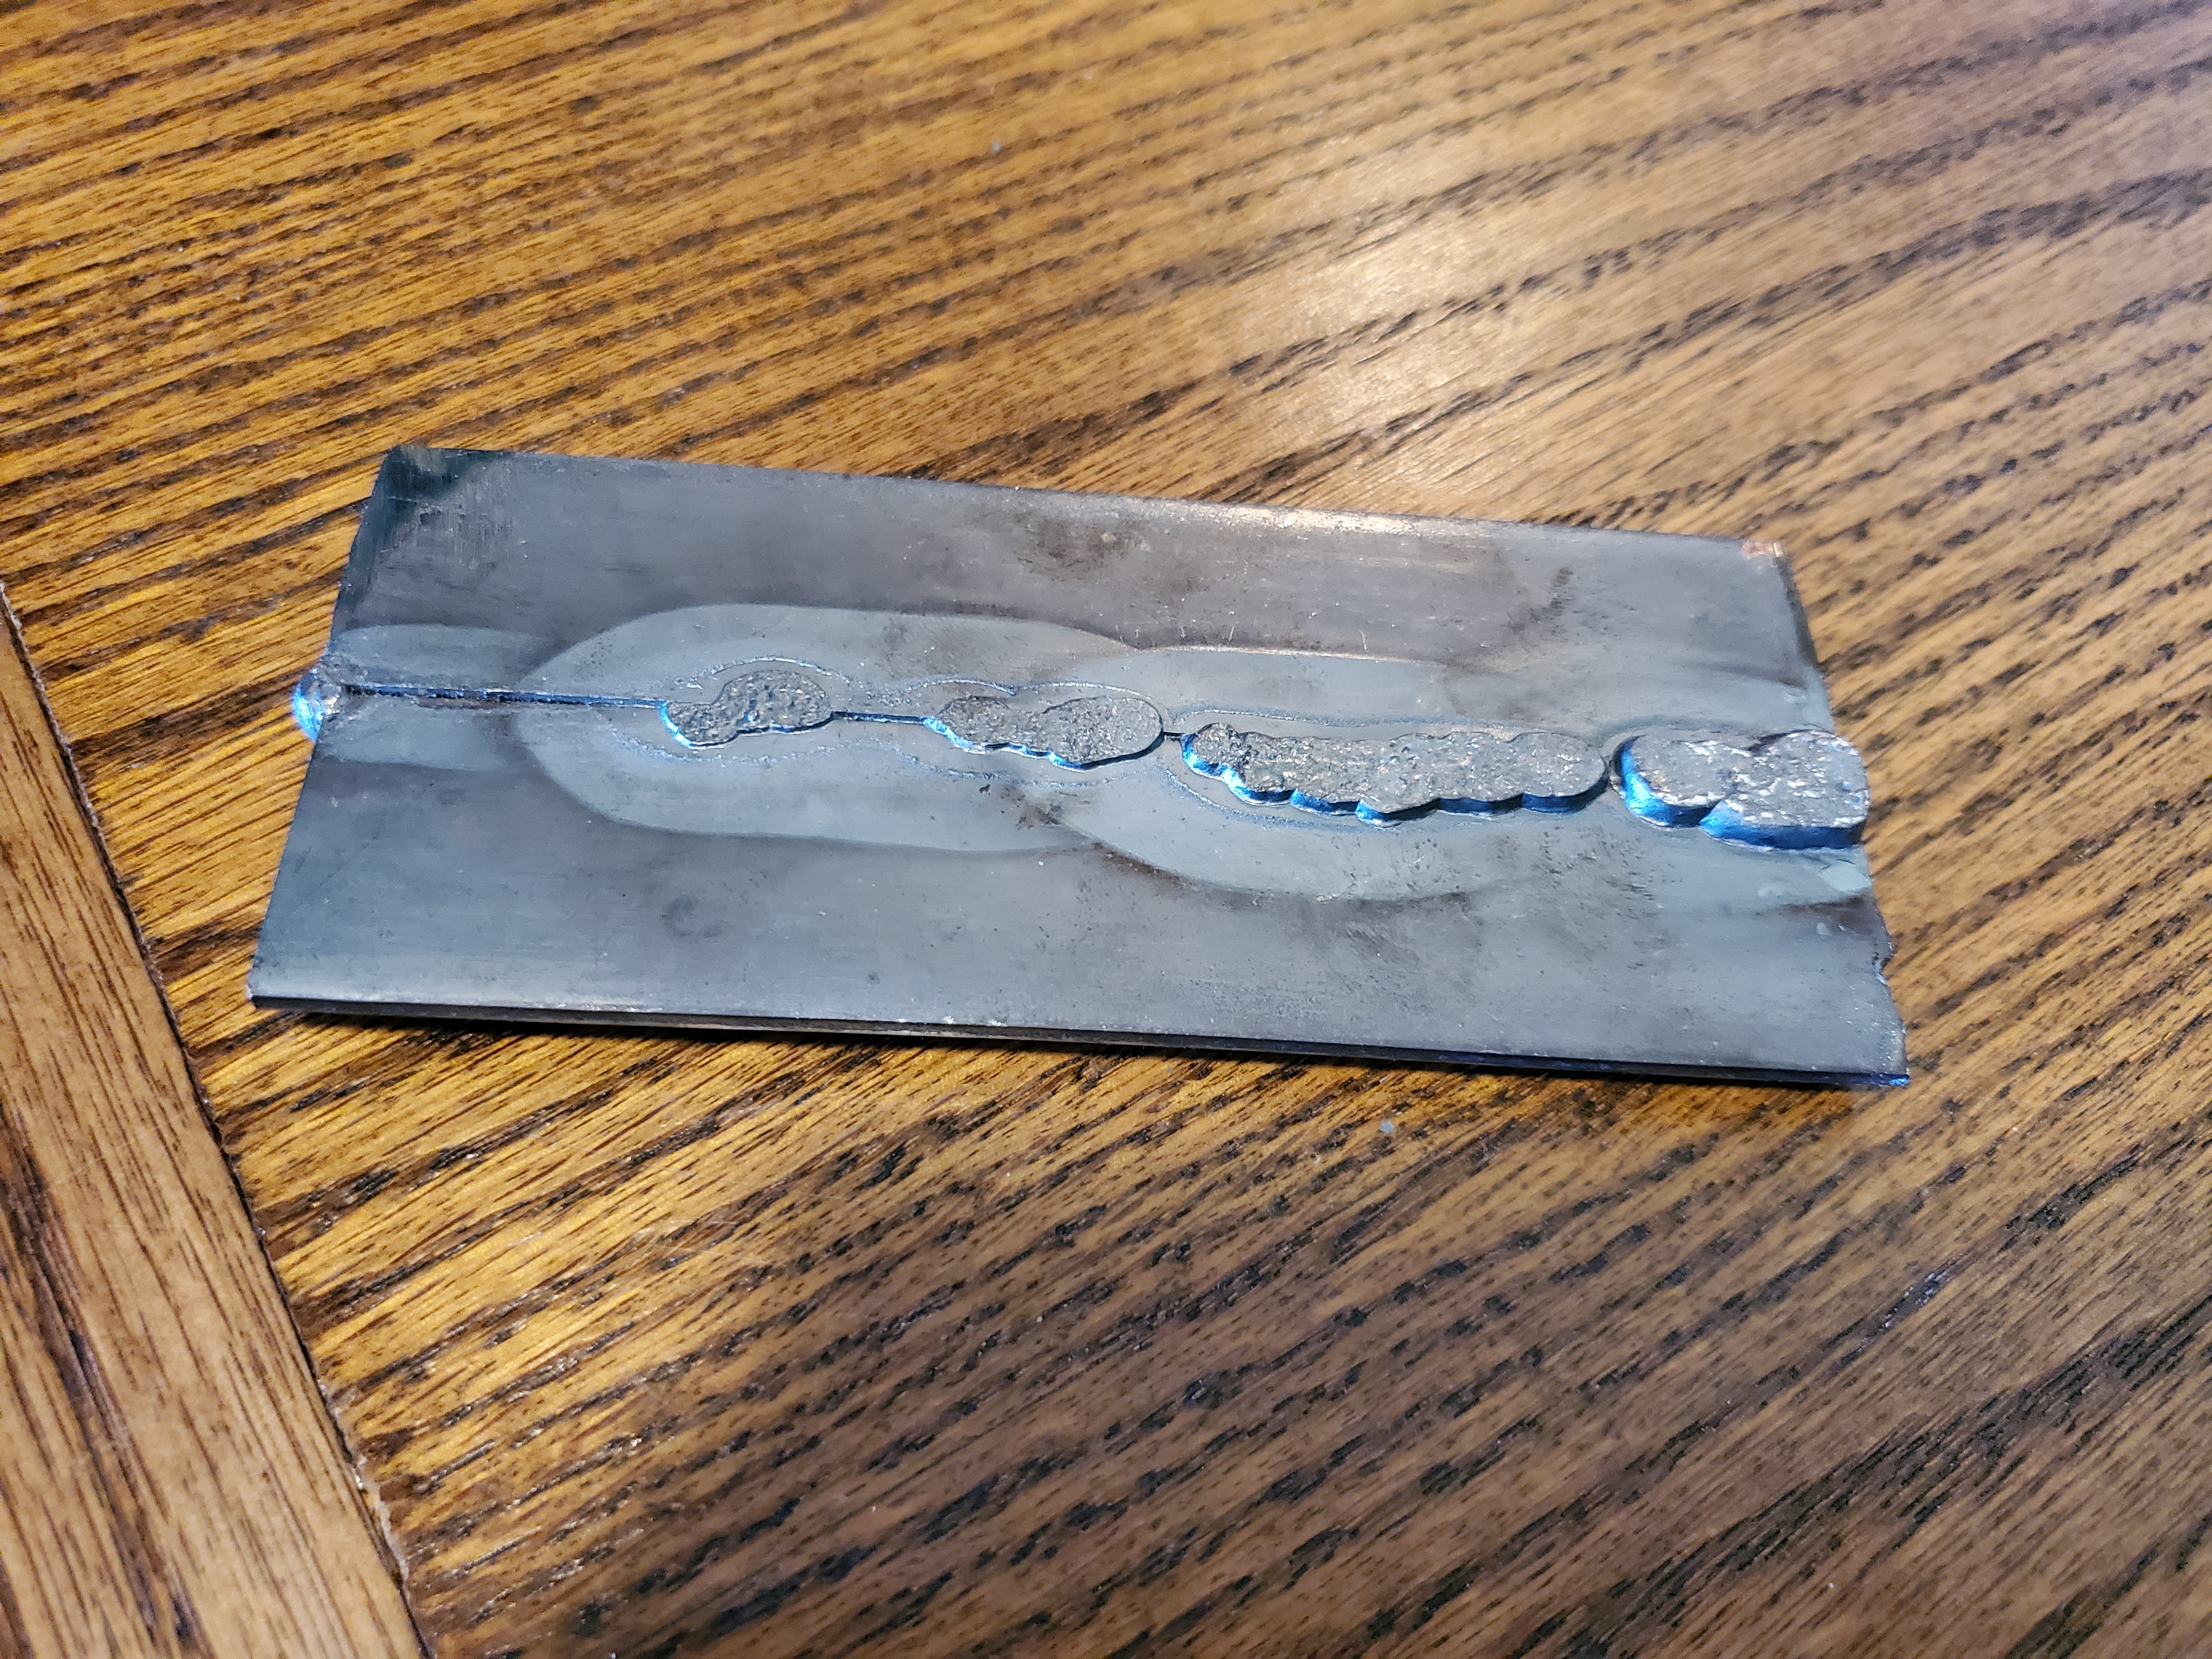
\includegraphics[width=\textwidth]{assets/buttWeldBack_20240229.jpg}
\label{butt2}
\end{figure}

\subsection*{Corner Weld}

The corner weld was interesting and educational. Figure \ref{corner1} shows the inside where I made two tacks and welded between them. Note that the large blob on the left end is a ``blown-out'' corner from the other side, which I'll address shortly. I also didn't wholly weld through the tacks because I wanted to practice getting the angle of my wire correct, which was something I saw on \href{https://www.youtube.com/watch?v=kUDrP2_JJ68}{a ``Tim Weld's'' YouTube video}. Welding from left to right, I experienced four things. On my first run of about an inch, my wire was too long, and my angle was too steep. These are indicated by the hole in the middle of the weld and the material ``spilling over'' onto the bottom plate. My second run was OK - the angle was good, the rate was acceptable, and overall, it was pretty decent. However, on my third run, I changed my angle to a shallow one, which caused material to creep up the top plate.

Figure \ref{corner2} shows what happened when I flipped this piece and started to weld the back of the corner. The weld path goes from left to right. The lesson I learned here is that when the piece is already hot, adding more material can damage it. I should have let it cool, I think. In this case, the left corner blew out straight out and down onto the welding table after only a second of heat. As I moved down the piece, I could watch it collapse if I went too slowly. The weld improves near the middle because we lowered the voltage and the feed rate on the welder to compensate for the extra heat. I liked the behavior of the lowered settings so much that I kept them for the T-joint weld.

Figure \ref{corner3} shows the unwelded side of the piece. The weld path runs from right to left, and the blown-out corner is visible on the right. Two other collapsing spots are available in this view at about 1 inch and 1.5 inch from the right.

\begin{figure}[h]
\caption{The front/inside of my corner weld showing a blown out corner (see next picture), two tacks, and a weld path from left to right.}
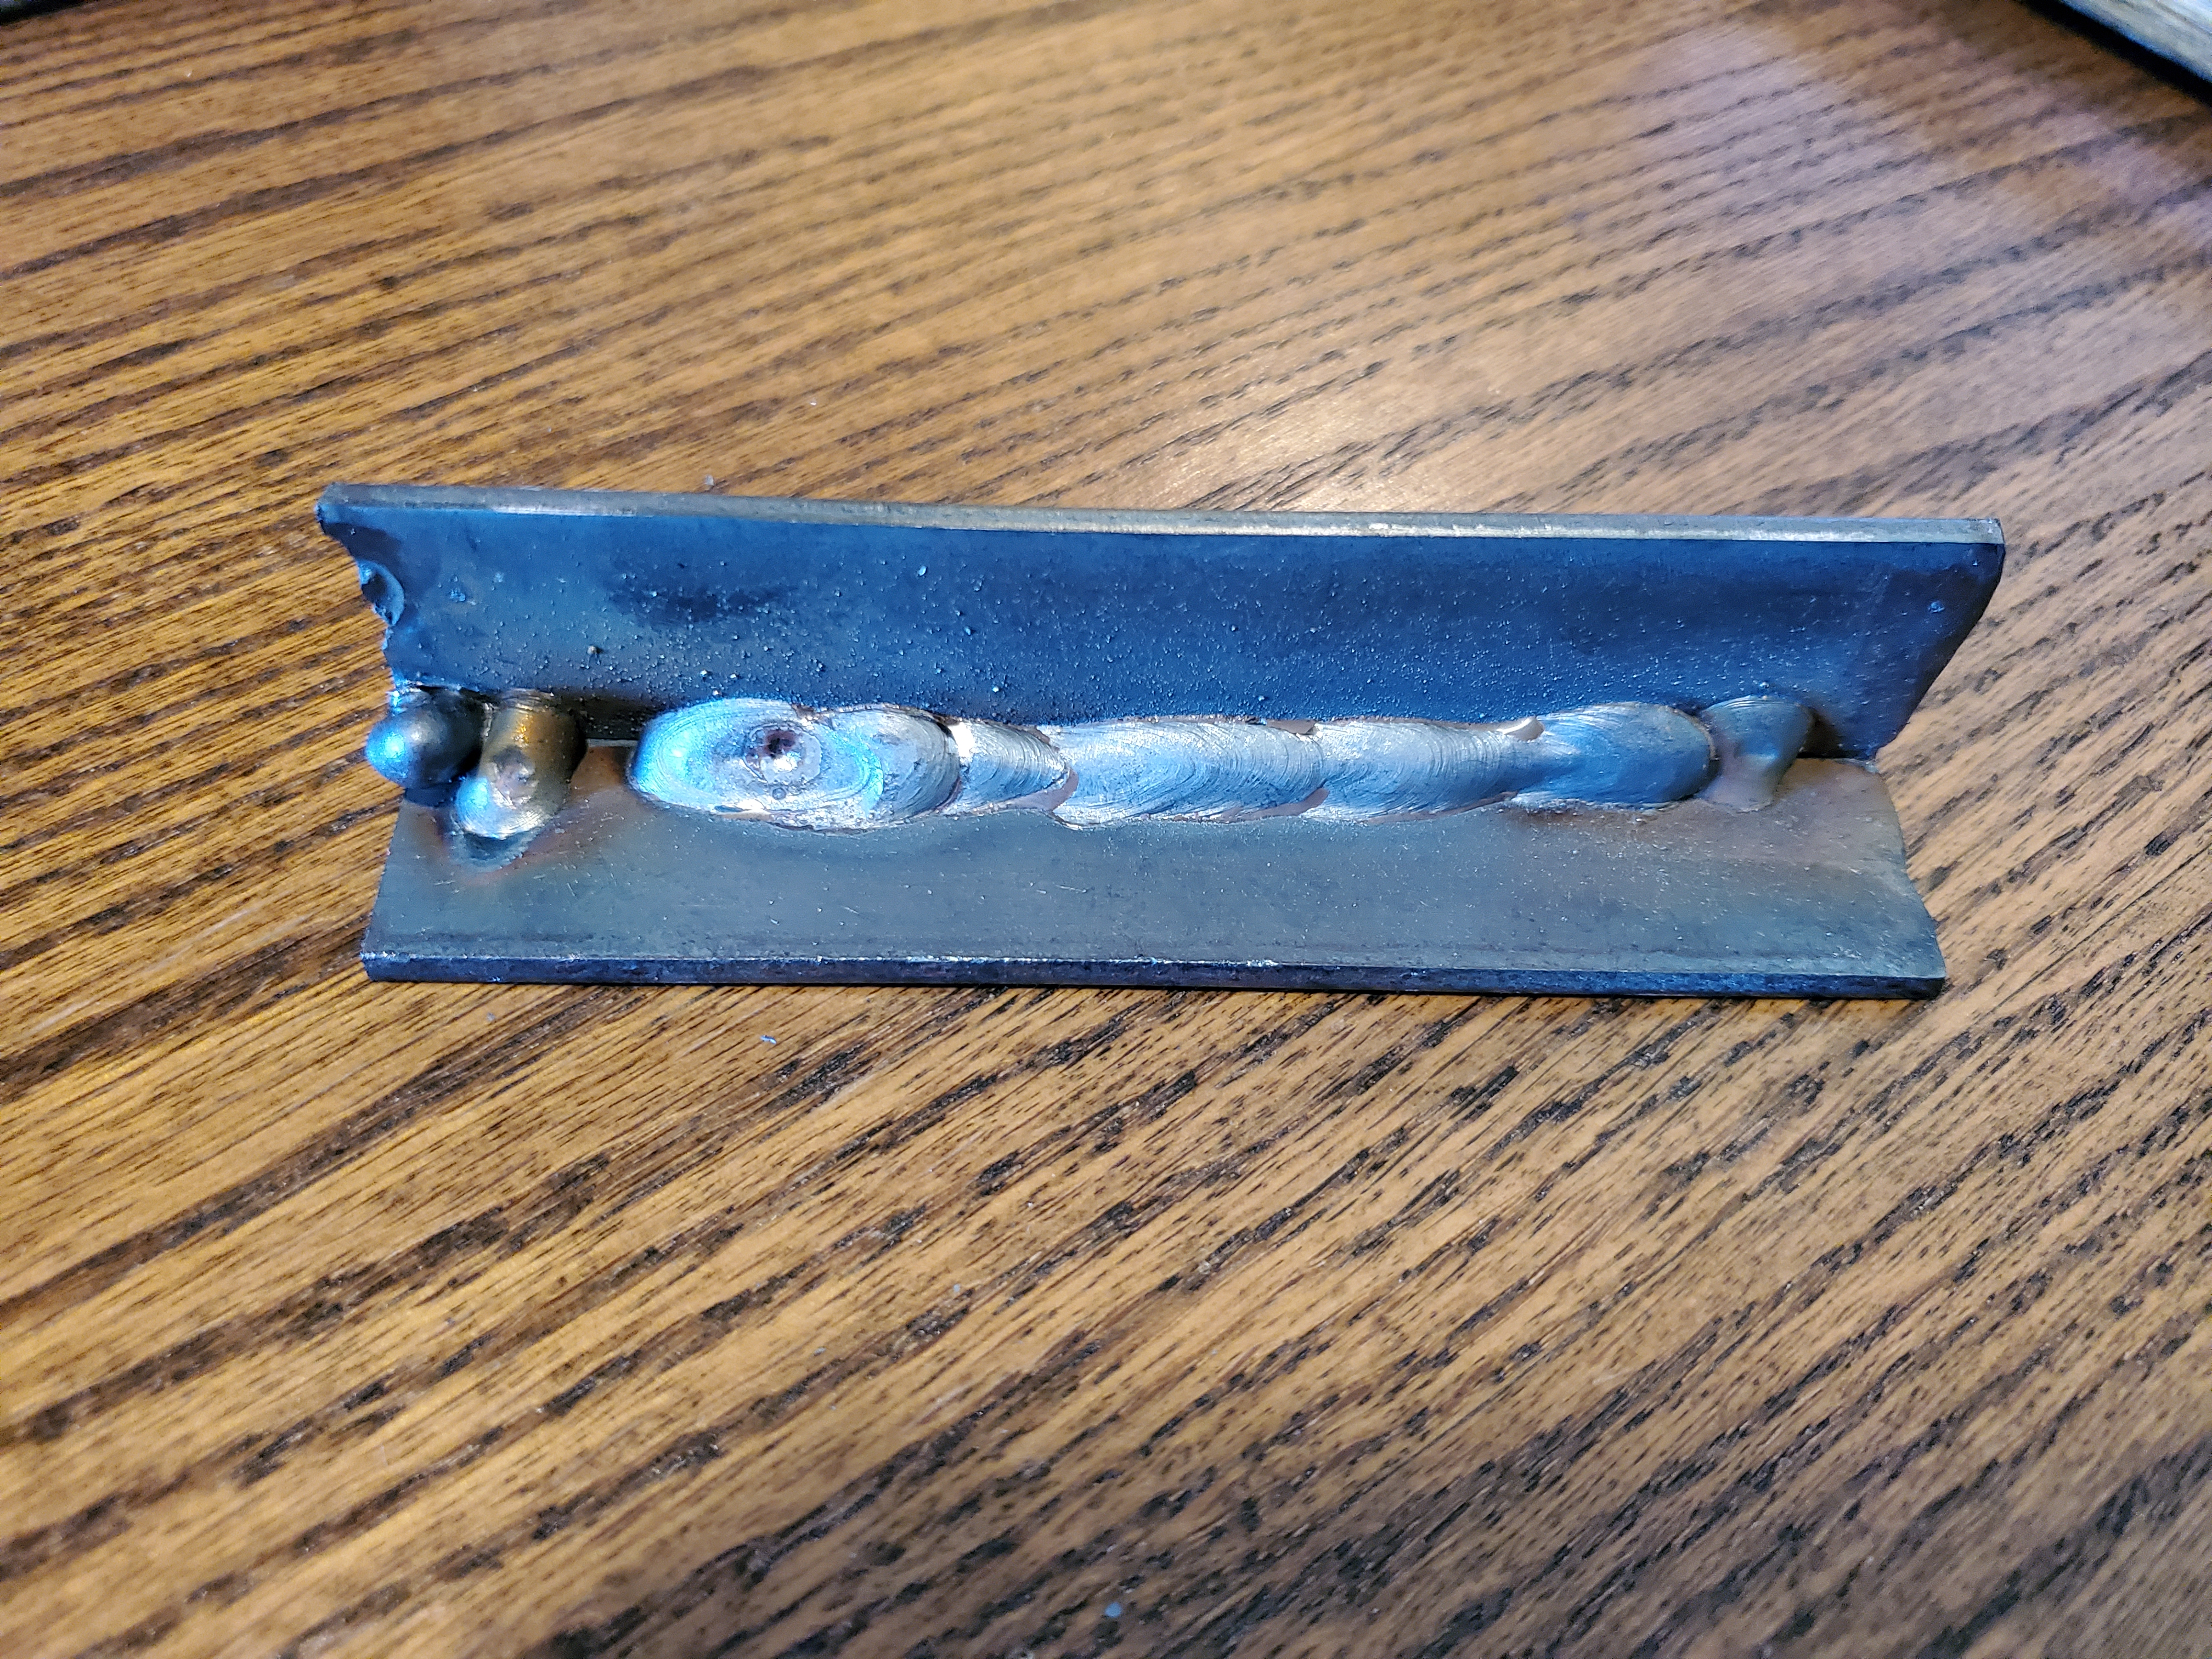
\includegraphics[width=\textwidth]{assets/cornerWeldFront_20240229.jpg}
\label{corner1}
\end{figure}

\begin{figure}[h]
\caption{The outside of the corner weld with the weld path going from left to right. The blown-out corner is visible on the left.}
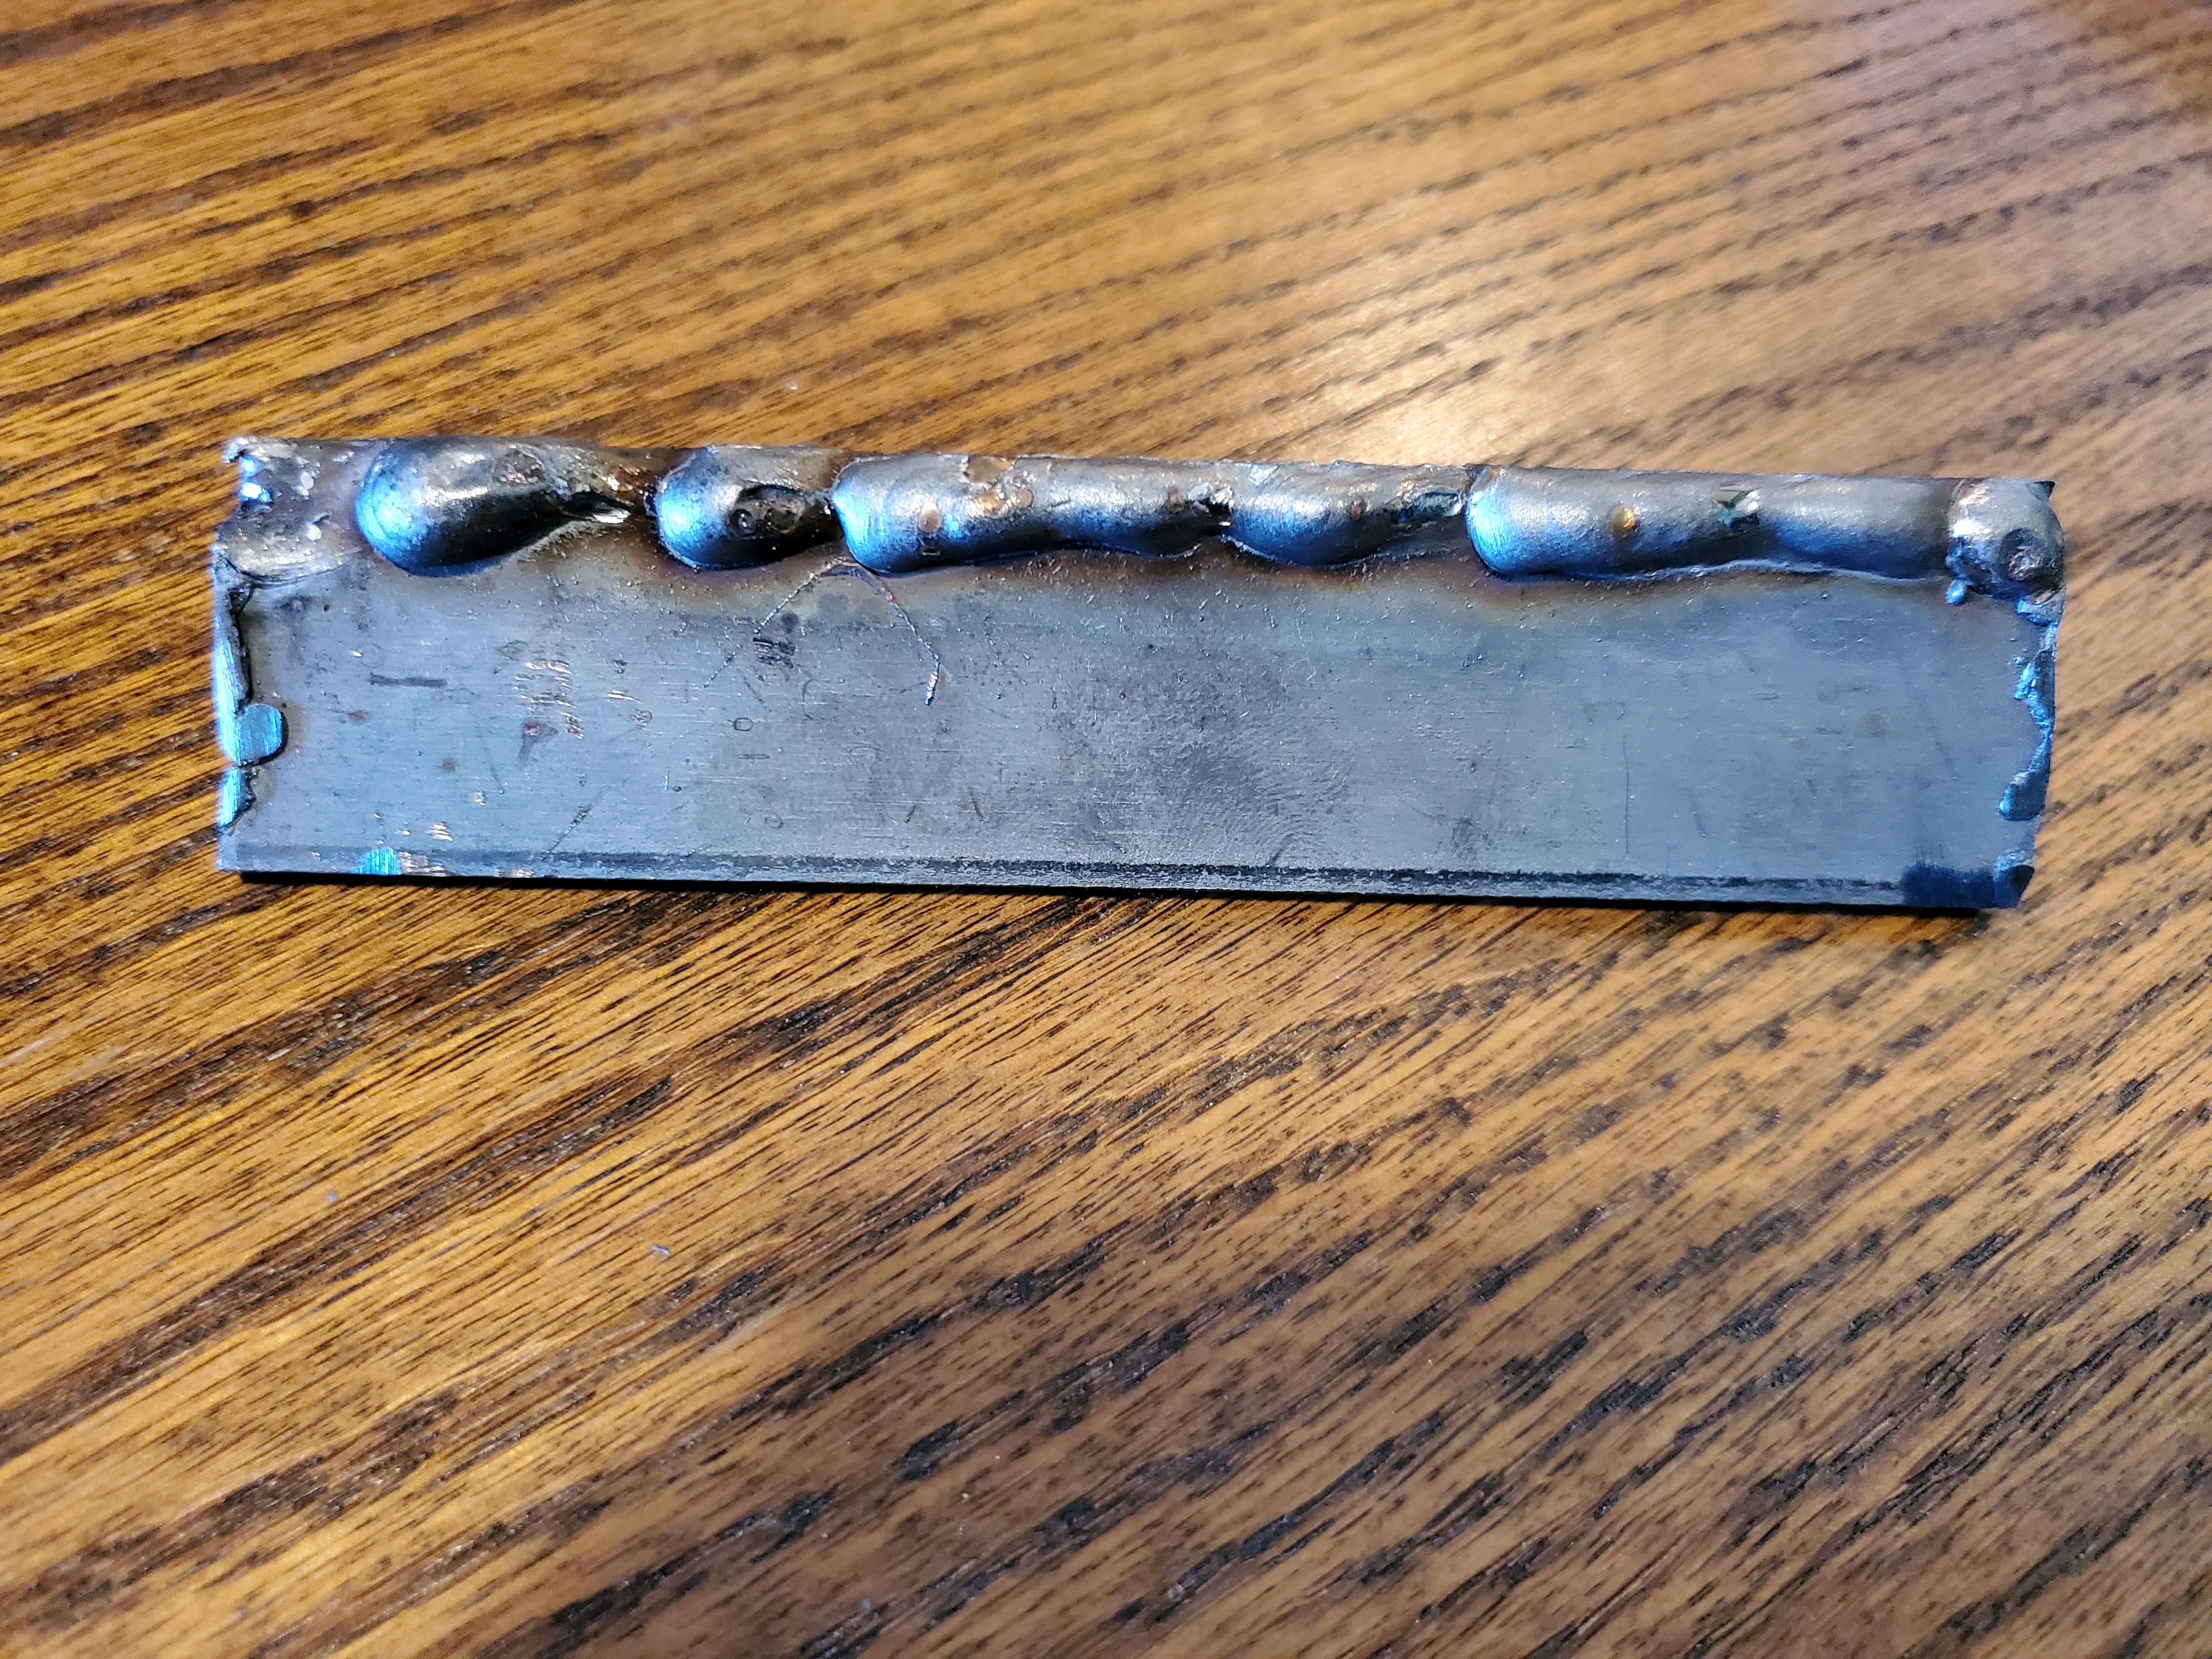
\includegraphics[width=\textwidth]{assets/cornerWeldOutside_20240229.jpg}
\label{corner2}
\end{figure}

\begin{figure}[h]
\caption{The third side of the corner weld with the weld path going from right to left.}
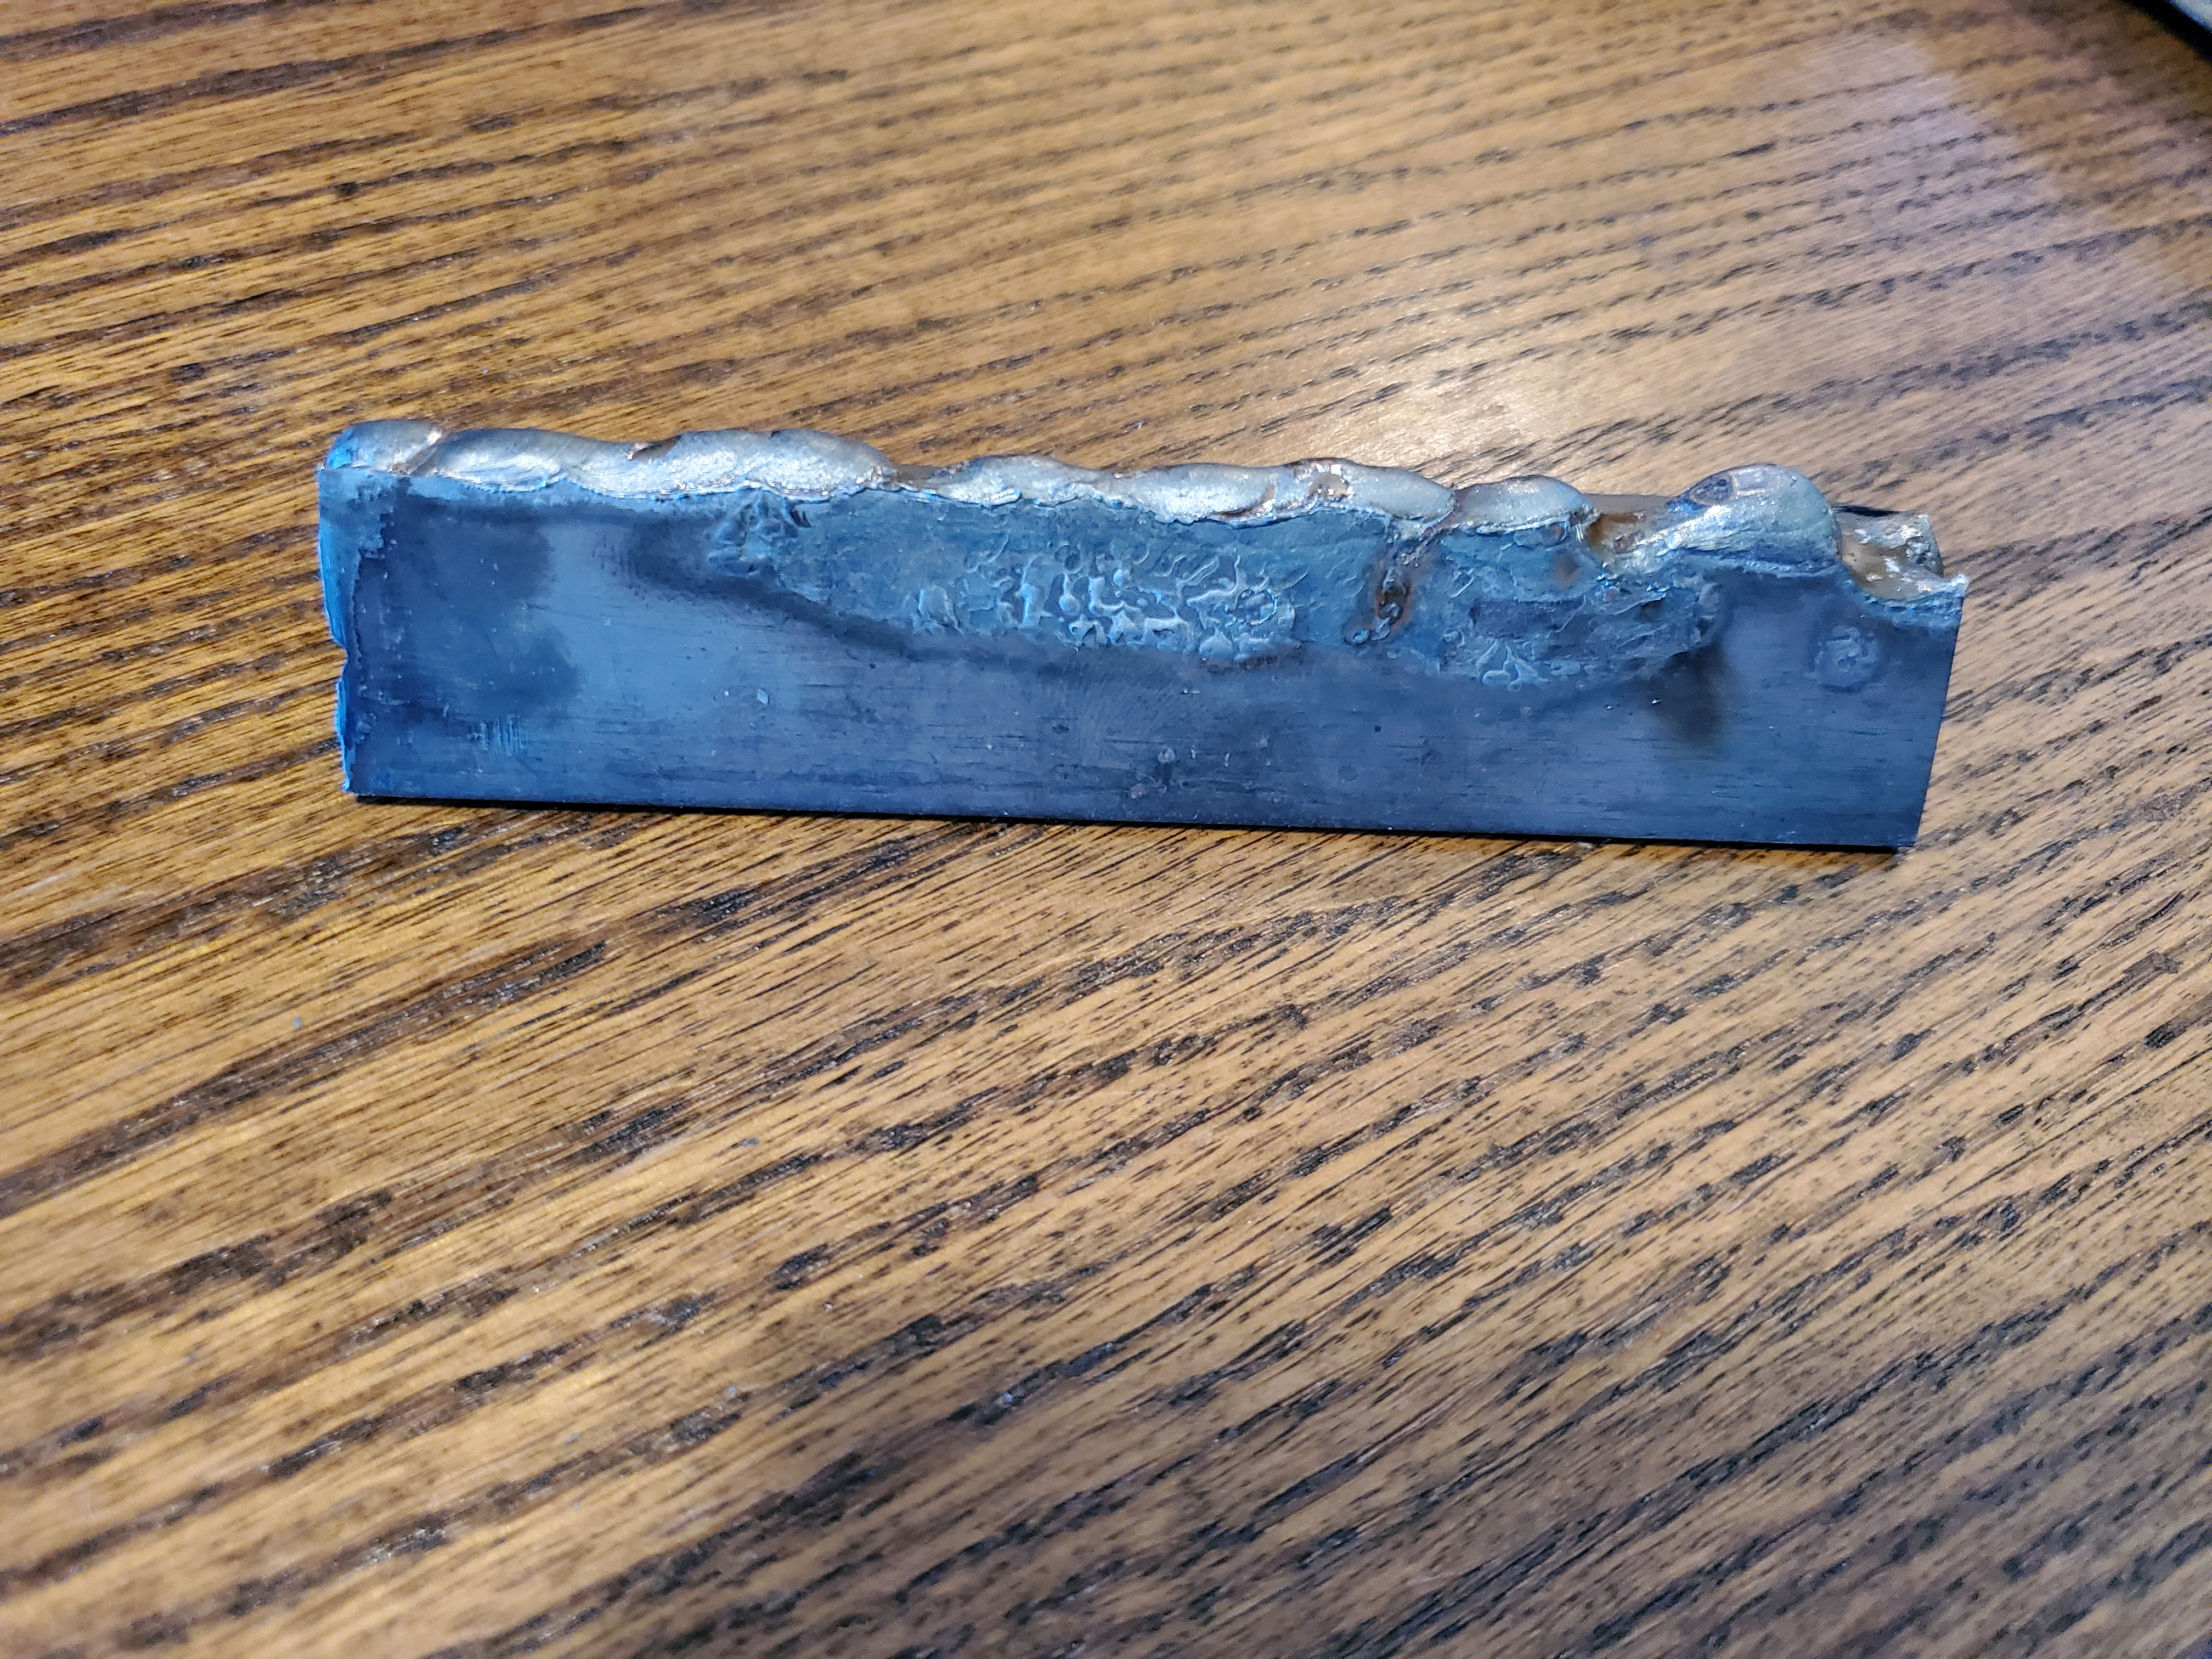
\includegraphics[width=\textwidth]{assets/cornerWeldOutside2_20240229.jpg}
\label{corner3}
\end{figure}

\subsection*{T-joint Weld}

I was pretty happy with my T-joint weld. I placed two tacks on the ends and proceeded to weld from end to end, left to right, crossing both tacks this time (figure \ref{tJoint1}). I burnt the left corner out a bit, but I practiced putting it back when I welded the back side by dragging the melt pool (figure \ref{tJoint2}). I'm not sure it worked, but it was fun to try. I also welded for lengths of 2-2.5 inches per attempt on the back.

\begin{figure}[h]
\caption{The front side of my T-joint weld with the weld path running left to right between two tacks.}
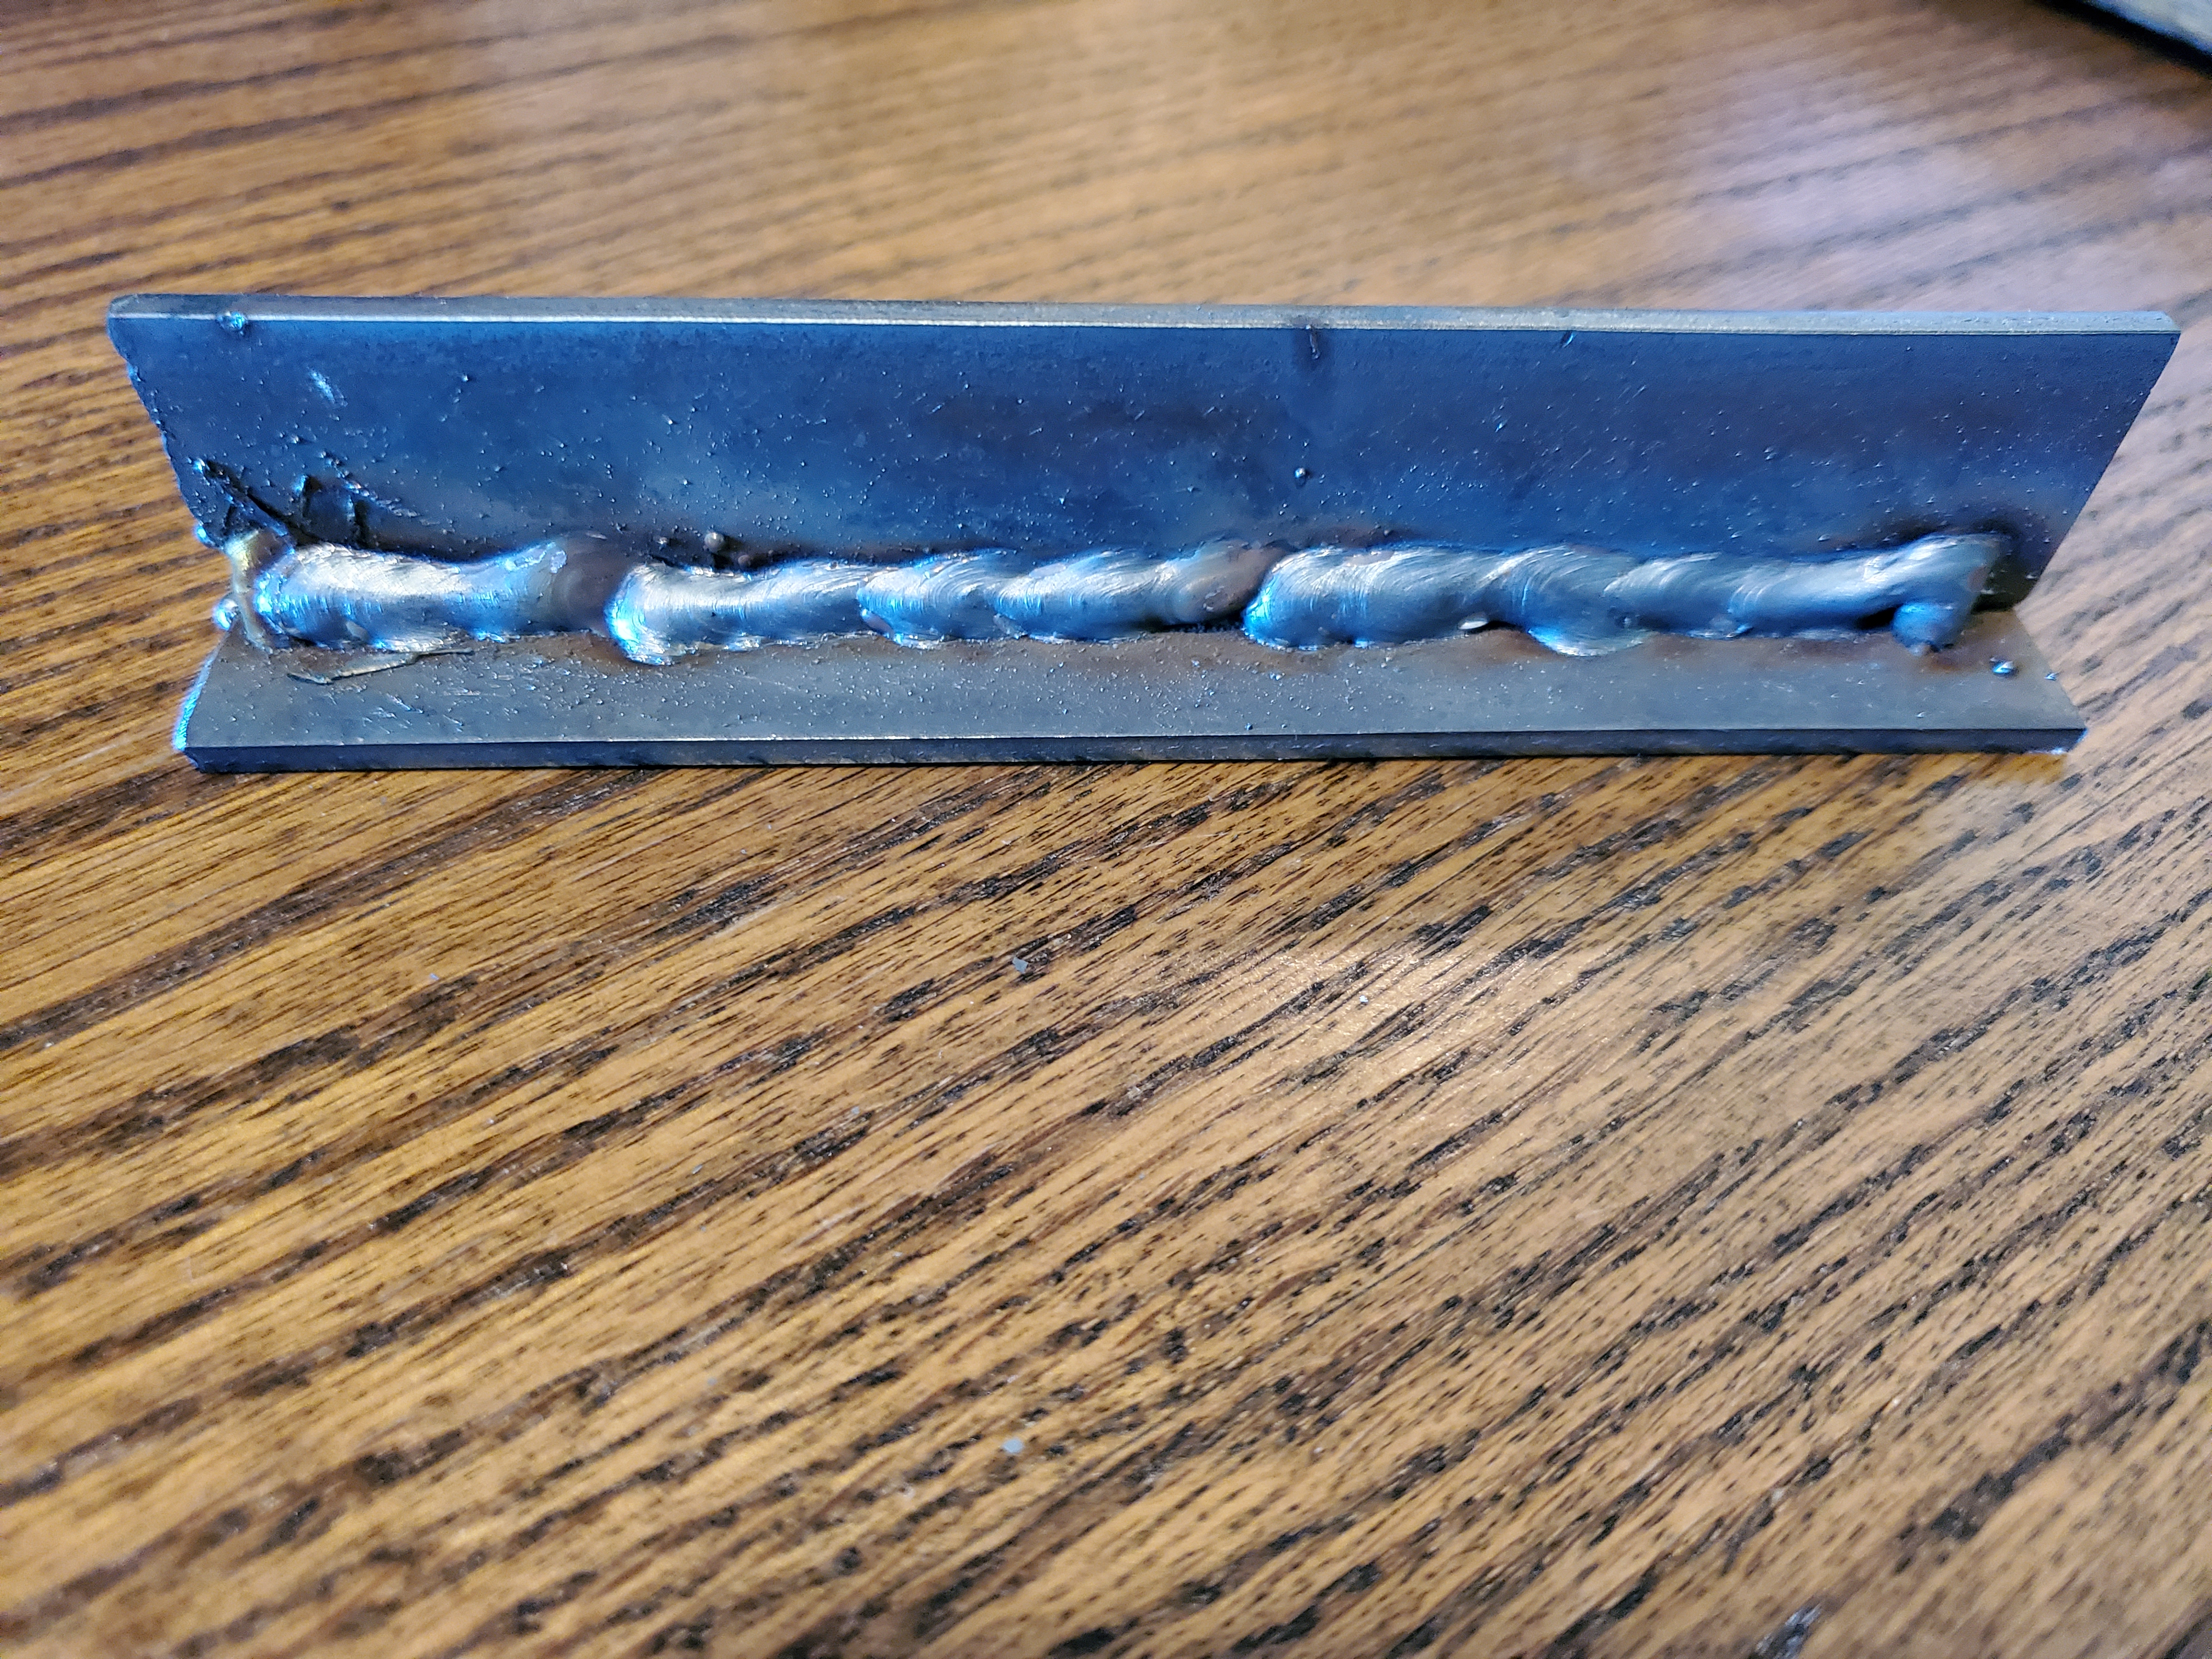
\includegraphics[width=\textwidth]{assets/tWeldFront_20240229.jpg}
\label{tJoint1}
\end{figure}

\begin{figure}[h]
\caption{The back side of my T-joint weld with the weld path running from left to right.}
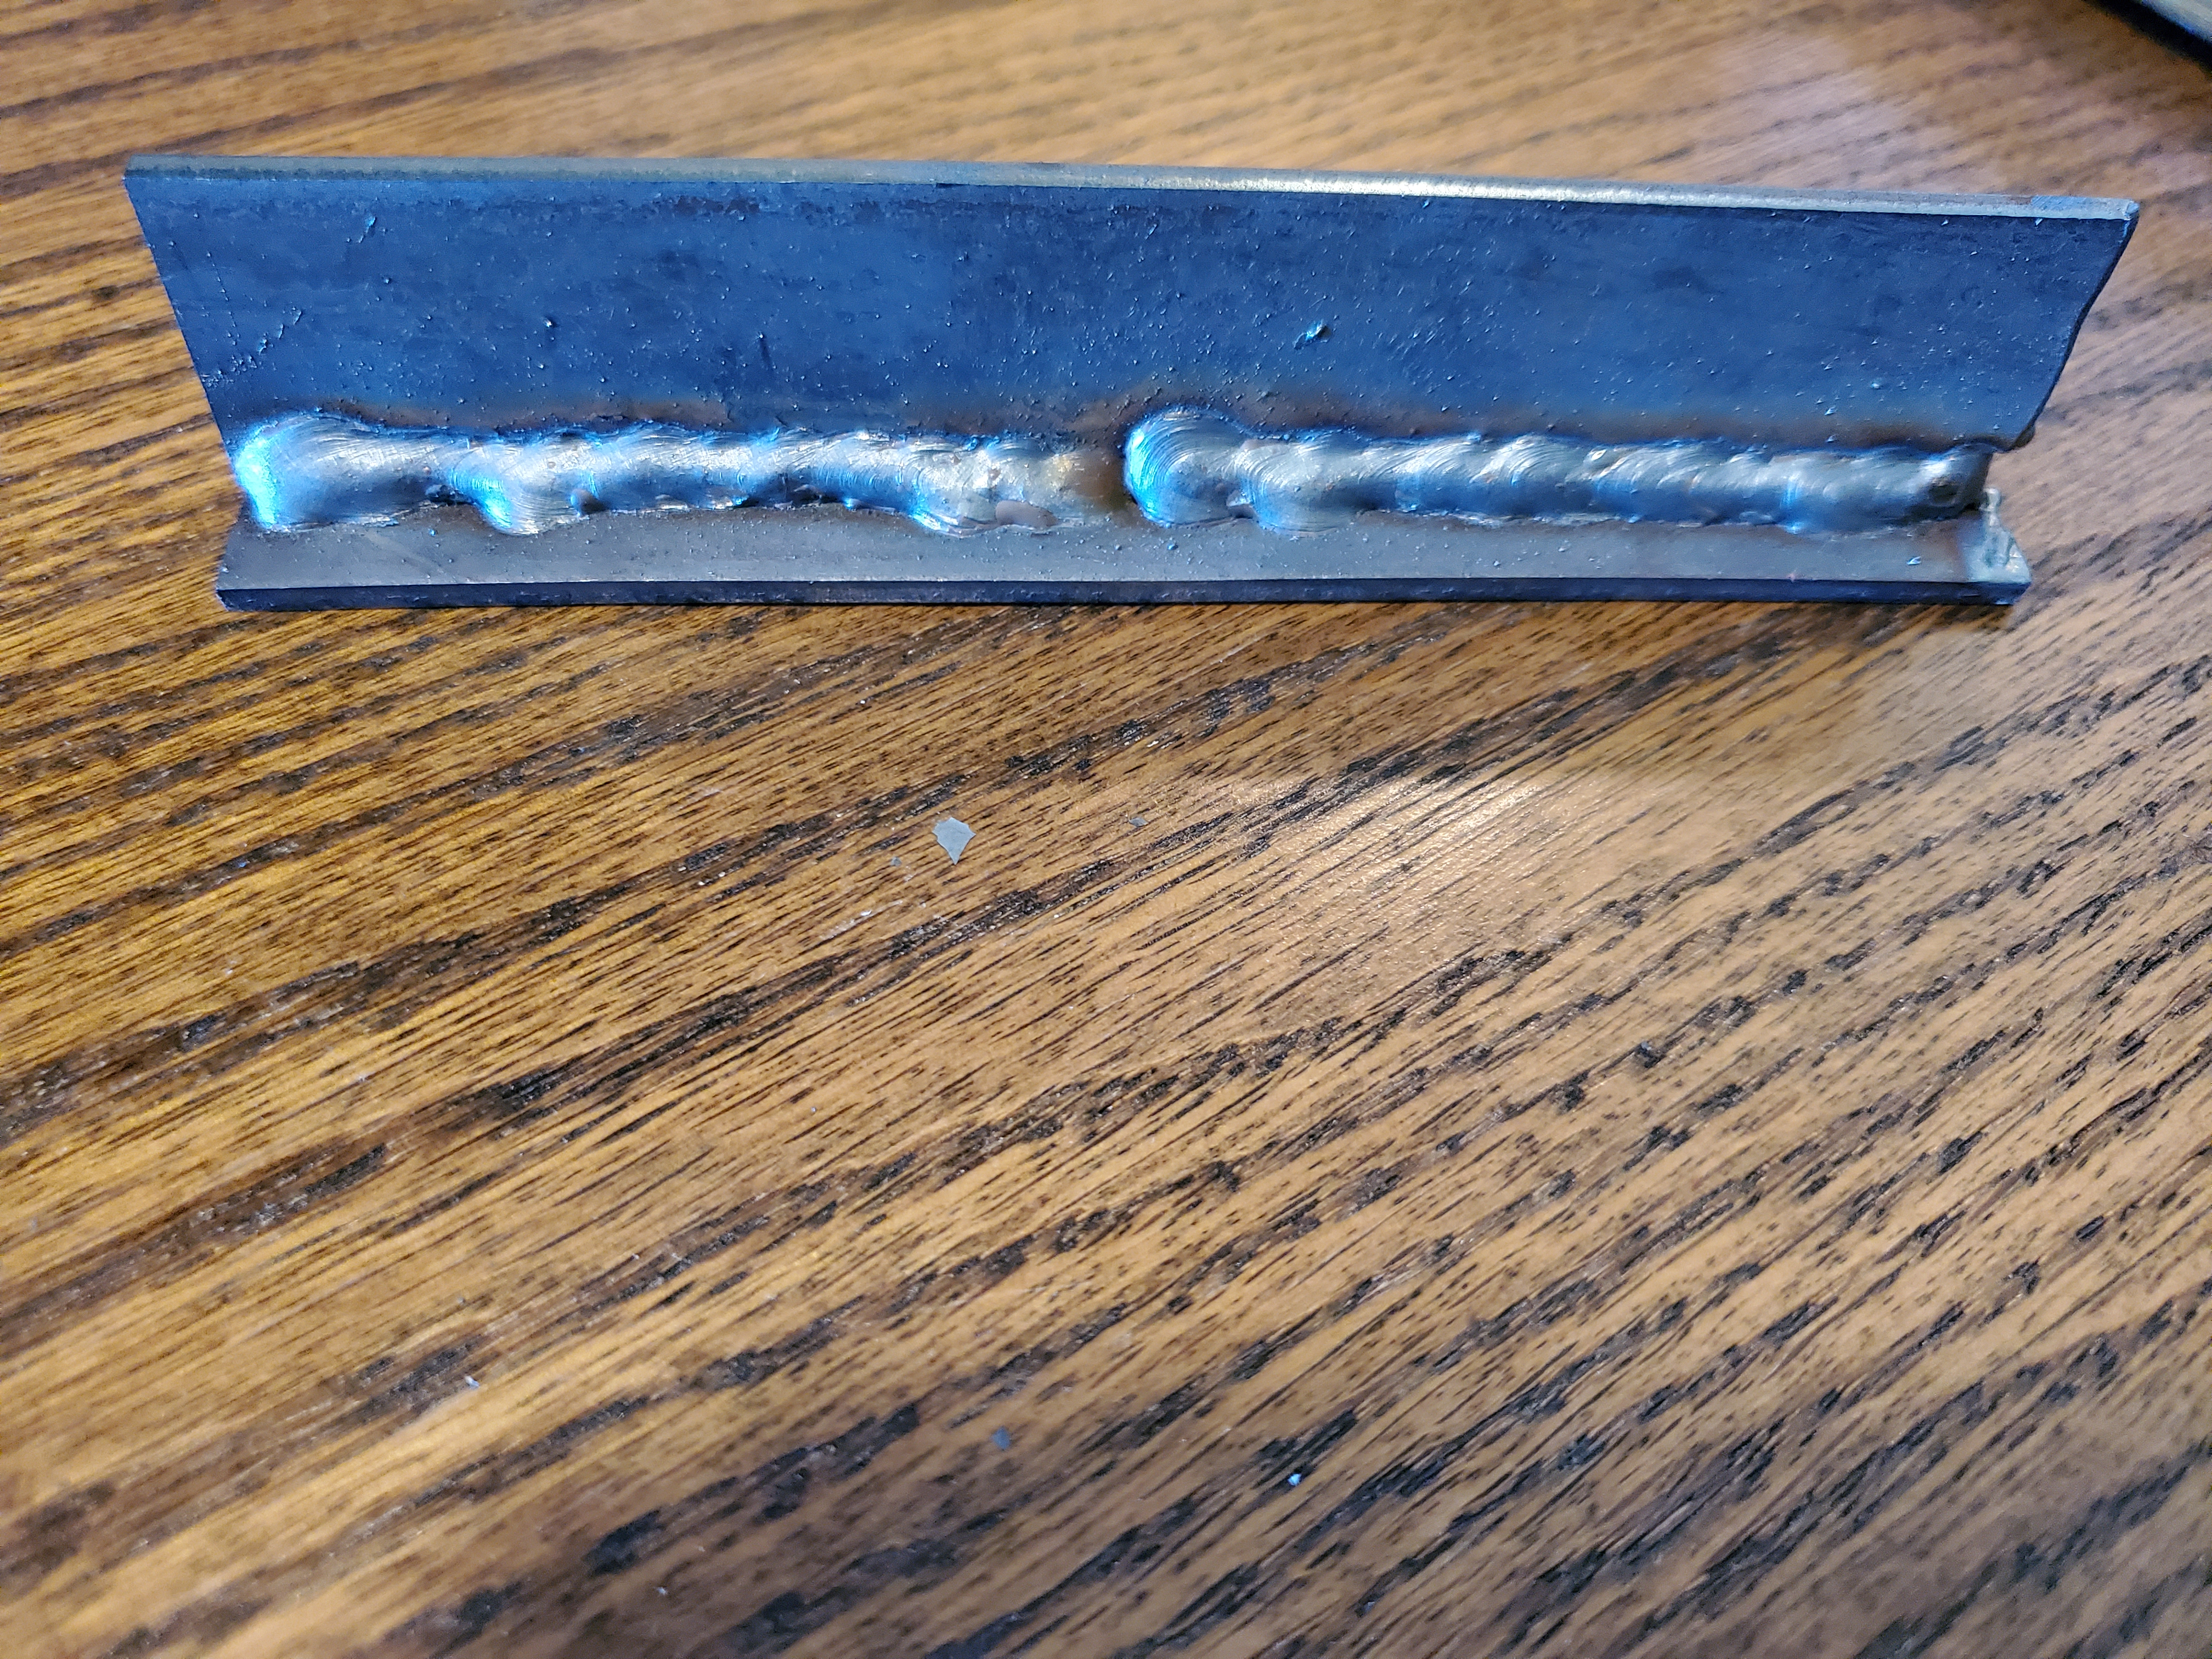
\includegraphics[width=\textwidth]{assets/tWeldBack_20240229.jpg}
\label{tJoint2}
\end{figure}

\section*{Final Thoughts}

I hope you enjoyed reading about my experience. I thought this was good fun, and I had to share. I had a wonderful time and learned so much from my instructor, Dilip Patel, to whom I will also say thank you very much!

What's next for me? I've got a ways to go before I weld a bridge! I passed my certification check with the welder on Saturday morning, so now I will order and make some coupons, then follow practice lessons from Tim Weld's.

I'd love to hear any tips, tricks, words of encouragement, suggestions, criticism, or funny jokes you have if you read this. Thanks so much, and have a great day!

\end{document}
